\documentclass[10pt,a4paper]{article}
\usepackage[latin1]{inputenc}
\usepackage{amsmath}
\usepackage{amsfonts}
\usepackage{amssymb}
\usepackage{float}
\usepackage{graphicx}
\begin{document}
\section{Descripci�n del problema.}
\section{Herramientas.}
Las herramientas que se pueden usar para abordar la resoluci�n del problema es amplia. Es por ello, que resulta dif�cil elegir la m�s adecuada. Tras un estudio de las bibliotecas disponibles para los distintos lenguajes de programaci�n que domino, me decante por weka(java),sklearn(python) y R. Para determinar cual de las 3 es la m�s conveniente en este caso, realizare pruebas de ejecuci�n de los diferentes algoritmos y compararemos el tiempo de ejecuci�n y el uso de memoria. Adem�s tendr� en cuenta la facilidad para tratar los datos y la biblioteca "en si". Los resultados obtenidos se muestran en las siguientes gr�ficas:	
\begin{figure}[!h]
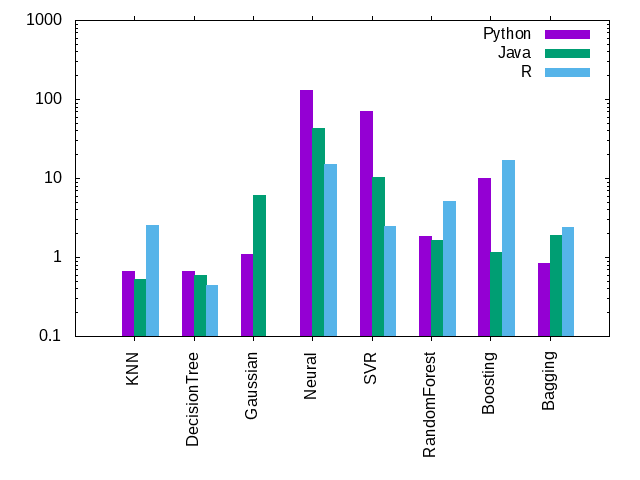
\includegraphics[scale=0.75]{./img/tiempos.png}
\end{figure}
\begin{figure}[H]
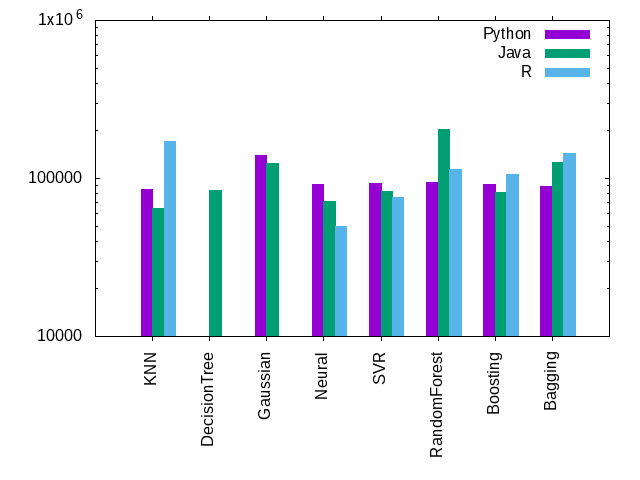
\includegraphics[scale=0.75]{./img/memoria.png}
\end{figure}

Observando los resultados podemos concluir que sklearn y weka ofrecen un rendimiento similar, mientras que R ofrece un mejor rendimiento para los algoritmos b�sicos pero es inferior en la ejecucion de multiclasificadores.
En cuanto al tratamiento de los datos tanto de lectura como para generar el archivo de resultados, tanto en R como en sklearn se hace de forma c�moda. Otra cuesti�n a tener en cuenta, es la buena documentaci�n con la que cuenta sklearn. Por tanto, poniendo en la balanza estos apuntes me decanto por Python como lenguaje a usar.

En particular, se usaran las siguientes bibliotecas:
\begin{itemize}
\item NumPy.
\item Pandas.
\item Scikit Learn.
\item XGBoost.
\end{itemize}
\section{Algoritmos.}
A priori desconocemos que algoritmo se adapta mejor a nuestro problema, es por ello que realizaremos un estudio comparando varios algoritmos. Los algoritmos elegidos son los siguientes:
\begin{itemize}
	\item algoritmos b�sicos como KNN,Linear Regression y Arboles de regresion
	\item  algoritmos potentes como NeuralNetwork,Gaussian y SVM
	\item multiclasificadores como Random Forest, Boosting y Bagging
\end{itemize} En la siguiente gr�fica se muestran los resultados obtenidos.
\begin{figure}[H]
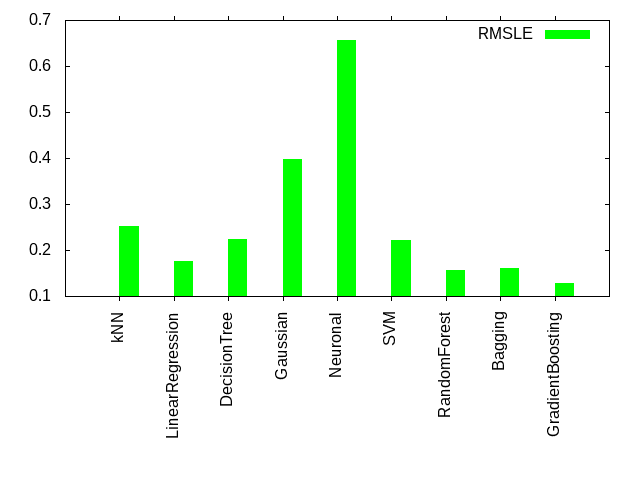
\includegraphics[scale=0.75]{./img/error.png}
\end{figure}
Se puede observar que los algoritmos que menor error proporcionan son los multiclasificadores. Por tanto, al igual que los competidores, nos decantamos por esta opci�n.
\end{document}